\documentclass[11pt,a4paper]{article}
% ---------------------------------------------------------------------
%  TFPT --- The frontier items: eta_B, m_p/m_e, Koide, dark matter, quantum gravity
%  Honest status: the genuine handle, the precision, and what is NOT a clean ladder.
%  No fabricated compiler rungs.  All numbers machine-verified.
% ---------------------------------------------------------------------
\usepackage[T1]{fontenc}
\usepackage[utf8]{inputenc}
\usepackage[english]{babel}
\usepackage{lmodern}
\usepackage[a4paper,margin=2.3cm]{geometry}
\usepackage{amsmath,amssymb}
\usepackage{booktabs,array,tabularx}
\usepackage{enumitem}
\usepackage{xcolor}
\usepackage{tikz}
\usetikzlibrary{positioning,arrows.meta}
\usepackage[most]{tcolorbox}
\usepackage{microtype}
\usepackage[hidelinks,colorlinks=true,linkcolor=blue!55!black,urlcolor=blue!55!black]{hyperref}
\emergencystretch=3em

\definecolor{tfblue}{HTML}{1F4E79}
\definecolor{tfgreen}{HTML}{1E7B45}
\definecolor{tfred}{HTML}{9B2226}
\definecolor{tfgold}{HTML}{B8860B}

\newtcolorbox{keybox}[1][]{enhanced,breakable,colback=tfblue!5!white,colframe=tfblue,fonttitle=\bfseries,coltitle=white,title={#1}}
\newtcolorbox{winbox}[1][]{enhanced,breakable,colback=tfgreen!6!white,colframe=tfgreen!75!black,fonttitle=\bfseries,coltitle=white,title={#1}}
\newtcolorbox{gapbox}[1][]{enhanced,breakable,colback=tfred!5!white,colframe=tfred!80!black,fonttitle=\bfseries,coltitle=white,title={#1}}

\newcommand{\tI}{{\small\textcolor{tfgreen}{\textbf{[I]}}}}
\newcommand{\tL}{{\small\textcolor{tfblue}{\textbf{[L]}}}}
\newcommand{\tF}{{\small\textcolor{tfgreen!45!black}{\textbf{[F]}}}}
\newcommand{\tN}{{\small\textcolor{tfgreen}{\textbf{[N]}}}}
\newcommand{\tP}{{\small\textcolor{tfgold}{\textbf{[P]}}}}
\newcommand{\tA}{{\small\textcolor{tfred}{\textbf{[A]}}}}
\newcommand{\markerkey}{\par\vspace{1.5pt}\noindent{\scriptsize\itshape\textcolor{black!58}{Marker key:\ \tI~exact identity\,$\cdot$\,\tL~Lie/lattice theorem\,$\cdot$\,\tF~formalised\,$\cdot$\,\tN~numerical fixed point\,$\cdot$\,\tP~physical/conditional\,$\cdot$\,\tA~axiom\,/\,open.}}\par\vspace{2pt}}
% inline reference to the script that machine-checks a claim (see verification/)
\newcommand{\veri}[1]{\,{\footnotesize\textcolor{tfblue!70!black}{[\,\texttt{verification/#1}\,]}}}
\newcommand{\phiz}{\varphi_0^{\mathrm{ret}}}
\newcommand{\cthree}{c_3}
\newcommand{\Mpl}{M_{\mathrm{Pl}}}
\newcommand{\Nfam}{N_{\mathrm{fam}}}
\newcommand{\Z}{\mathbb{Z}}
\setlist{itemsep=2pt,topsep=3pt}
\newcolumntype{Y}{>{\raggedright\arraybackslash}X}

\title{\vspace{-1.2cm}\textbf{TFPT --- Frontier items}\\[2mm]
\large $\eta_B$, $m_p/m_e$, the Koide relation, dark matter and quantum gravity ---\\
the honest status, not forced onto the ladder}
\author{}\date{\today}

\begin{document}
\maketitle
\vspace{-0.6cm}

\begin{keybox}[What this document is about --- the status authority for the frontier]
The honest frontier: which physics has a genuine TFPT handle and which does not. For each of
$\eta_B$, $m_p/m_e$, the Koide relation, dark matter and full quantum gravity, this note states the
genuine structural handle, the precision with which it currently lands, and --- crucially --- what is
\emph{not} a clean compiler power and is deliberately \emph{not} forced onto the ladder. \textbf{This
document is the status authority for the frontier items:} where any other document's wording and the
markers here disagree, the typing here (and the \texttt{status\_ledger.csv}) wins.
\end{keybox}

\begin{keybox}[The TFPT document set --- what is treated where]
\textbf{Plain language:} TFPT is a small discrete compiler. Two inputs --- the seam constant
$c_3=\tfrac1{8\pi}$ and the carrier rank $g_{\mathrm{car}}=5$ --- build $D_5\oplus A_3+\mu_4\Rightarrow E_8$
and read off the Standard Model, the constants and the scale grammar. The development is \textbf{six short
documents}, best read in order:
\begin{enumerate}[leftmargin=1.7em,itemsep=1pt]
\item \texttt{introduction} --- reading guide, compiler closure, paper-by-paper comparison, predictions, the dependency DAG and proof ledger.
\item \texttt{tfpt\_1\_architecture\_e8} --- the two axioms, the derivation map, the EM fixed point $\alpha^{-1}$, the $D_5\oplus A_3+\mu_4\Rightarrow E_8$ construction.
\item \texttt{tfpt\_2\_standard\_model} --- the SM in one $\varphi_0$-ladder formula, flavor from parabolic transport, the worked closures, and gravity/QG as the seam response.
\item \texttt{tfpt\_3\_e8\_audit\_bootstrap} --- the seven $E_8$ slices as an audit raster, the cascade bridge, the M\"obius bootstrap.
\item \texttt{tfpt\_4\_frontier} --- honest status of $\eta_B$, $m_p/m_e$, Koide, dark matter, full QG.
\item \texttt{tfpt\_horizon\_readouts} --- one seam constant as the universal horizon thermal code.
\end{enumerate}
\textbf{You are reading document \#5.}
\end{keybox}

\tableofcontents
\bigskip

\begin{gapbox}[Ground rule]
These five are exactly the items previously flagged ``\emph{not on a clean action/ladder yet --- do not
force}.'' This note gives, for each, the \emph{genuine} structural handle that does exist, the precision
with which it currently lands, and a clear statement of what is \emph{not} a single compiler power. No
fabricated ladder rungs; the honest markers \tI/\tP/\tA\ are applied throughout. (All numbers
machine-verified.)
\end{gapbox}

\begin{gapbox}[Hard rule on the frontier ($F_{\mathrm{frontier}}$)]
\textbf{Koide, $\eta_B$, the axion relic scale and $m_p/m_e$ are \emph{not} compiler powers unless their
missing QFT-transfer / cosmology computation is explicitly supplied.} They are deliberately typed
interfaces, not structural holes: each has a genuine handle (a near-value, a determined readout, a fixed
candidate) but its \emph{exact} status is conditional on a named, not-yet-performed calculation (the
source$\to$pole QFT shift; the flavored-leptogenesis Boltzmann solve; the near-hilltop relic integral with
anharmonic/string corrections; the QCD/EW cross-sector matching). They must never be quoted as primitive
TFPT outputs.

\smallskip
\noindent\emph{Why this is principled, not a gap:} these are precisely the \textbf{discrete$\leftrightarrow$
continuous boundary} of the theory --- the points where the discrete compiler hands its skeleton off to
continuous physics (QCD confinement, cosmological Boltzmann transport, relic integrals). The cleanness of a
quantity tracks how far it sits from that handoff: pure compiler ratios are exact, QCD/cosmology-dressed
quantities are typed interfaces. \veri{v35\_quark\_qcd\_boundary.py}
\end{gapbox}

% =====================================================================
\section{Baryon asymmetry $\eta_B$ --- a downstream readout from the closed $\Omega_b h^2$}
% =====================================================================
There are two independent handles, and they agree.

\paragraph{Route A --- from the closed baryon fraction.} The seed already fixes the baryon
\emph{fraction} (Paper 3 decoder):
\[
  \Omega_b=(4\pi-1)\beta_{\mathrm{rad}}=\Bigl(1-\tfrac1{4\pi}\Bigr)\phiz=0.04894 ,\qquad
  \beta_{\mathrm{rad}}=\frac{\phiz}{4\pi},
\]
matching the observed $\Omega_b\approx0.049$. The baryon-to-photon ratio is then the \emph{standard}
cosmological readout $\eta_B=273.9\times10^{-10}\,\Omega_b h^2$. With the TFPT Hubble value
($h\approx0.674$, from $H_0\sim\sqrt\Lambda$),
\[
  \boxed{\ \Omega_b h^2=0.0222,\qquad \eta_B=6.09\times10^{-10}\ }\qquad(\text{observed }6.1\times10^{-10}).
\]
So $\eta_B$ is a \emph{downstream cosmological readout} from the closed $\Omega_b h^2$ handle --- not an
independent compiler rung, and the fundamental leptogenesis route remains an interface.

\paragraph{Route B --- leptogenesis interface (Paper 6, \tI).} The closed branch also fixes the
leptogenesis inputs: the heavy scale $M_R\approx1.3\times10^{15}$ GeV, the CP phases ($\delta_{\mathrm{CKM}}$,
$\delta^\nu_{\mathrm{CP}}$, both closed), the reheating $T_R$, and the seam-fixed initial phase. The
numerical $\eta_B$ then follows from the \emph{standard} flavored-leptogenesis Boltzmann solve --- an
independent cross-check of Route A. \textbf{Honest caveat:} that Boltzmann network (the
washout/efficiency $\kappa_f$, the flavored density-matrix equations) is the standard leptogenesis
machinery (Davidson--Nardi--Nir, \emph{Phys.\ Rep.}\ 466 (2008) 105; Buchm\"uller--Di~Bari--Pl\"umacher,
\emph{Ann.\ Phys.}\ 315 (2005) 305); it is \emph{not} carried out or attached here. Route~B is therefore a
\emph{named interface}, not a closed number; only Route~A (downstream of the closed $\Omega_b h^2$) is
quoted.

\begin{keybox}[Honest status of $\eta_B$ --- strictly typed \tP]
The two statements must be kept apart and not interchanged:
\[
  \boxed{\ \eta_B\ \text{as a cosmological readout from the closed }\Omega_b h^2\ \text{is \emph{determined}}\ (6.1\times10^{-10})\ }
\]
\[
  \boxed{\ \eta_B\ \text{as a fundamental \emph{compiler power} is \emph{not} closed}\ }
\]
The leptogenesis route requires a standard (washout-dependent) Boltzmann solve. So $\eta_B$ is \tP ---
determined as a downstream readout, but \emph{not} a clean compiler rung; it must never be quoted as a
fundamental TFPT output.
\end{keybox}

% =====================================================================
\section{Proton/electron ratio $m_p/m_e$ --- a cross-sector ratio}
% =====================================================================
$m_e$ is \emph{closed} on the $\phiz$-ladder ($\hat m_e=\tfrac{v_{\mathrm{geo}}\pi}{\sqrt2}\tfrac{16}{7}(\phiz)^5$).
The proton mass is \emph{not} a Yukawa: it is QCD-dominated, $m_p\sim$ a few $\times\Lambda_{\mathrm{QCD}}$,
and $\Lambda_{\mathrm{QCD}}$ arises by dimensional transmutation from $\alpha_s$ running (scheme level).
Hence
\[
  \frac{m_p}{m_e}=\frac{\text{QCD confinement scale}}{\text{EW electron Yukawa}}=1836.15
\]
mixes \emph{two different sectors}. It is no single $\phiz$ power: $1/(\phiz)^2=353.7$ and
$1/(\phiz)^3=6651$ bracket $1836$ with no clean rung in between.

\begin{keybox}[Honest status of $m_p/m_e$ \tA]
Computable at \emph{scheme level} (from $\alpha_s(M_Z)$ running $+$ the closed $m_e$), exactly like the
dimensionful EW/QCD masses $m_W,m_Z$. But it is \emph{genuinely not} a compiler power, because it is a
ratio across the QCD and electroweak sectors. Left \tA\ --- not forced.
\smallskip\\
\noindent\textbf{A rejected near-formula (recorded as a discipline boundary, \veri{v79\_review\_identities.py}).}
The combination $|W(D_5)|-\dim\Lambda^3(SU(9))+\Nfam\lambda_C^2=1920-84+0.151=1836.151$ matches the PDG value to
$\sim10^{-6}$ --- and is \emph{deliberately rejected}. Two reasons make it numerology, not a derivation:
$SU(9)=A_8$ (the $\dim\Lambda^3=84$ block) does \emph{not} occur in the carrier $D_5\oplus A_3$, and $m_p$ is
QCD confinement (gluon binding energy) with \emph{no} mechanism linking it to an algebraic sum. Integrating it
would \emph{invite} the numerology charge, not retire it; $m_p/m_e$ stays \tA. (The same firewall rejects
$\eta_B=\tfrac{|\Z_2|}{\Delta_Q}\cthree^6\approx6.10\times10^{-10}$: arithmetically close, but a two-atom
prefactor fit to a washout-dependent leptogenesis output --- $\eta_B$ stays \tP, the downstream readout above.)
\end{keybox}

% =====================================================================
\section{The Koide relation --- near $2/3$, computed exactly}
% =====================================================================
With the closed lepton source masses $\hat m_\ell\propto(\tfrac{16}{7}(\phiz)^5,\tfrac43(\phiz)^3,\tfrac76(\phiz)^2)$
the Koide ratio is a pure number (the common prefactor cancels):
\[
  Q_{\mathrm{TFPT}}=\frac{\sum_\ell \hat m_\ell}{\bigl(\sum_\ell\sqrt{\hat m_\ell}\bigr)^2}
  =0.66446\ldots,\qquad \frac23=0.66667,\qquad \text{deviation }-0.33\% .
\]
The measured pole-mass value is famously $Q_{\mathrm{PDG}}=0.66666$. So TFPT predicts a Koide ratio that
is \emph{near} $2/3$ but \emph{not exactly} $2/3$ at source level.

\begin{keybox}[Honest status of Koide \tP]
$Q_{\mathrm{TFPT}}=0.664$ is a \emph{prediction}, $0.33\%$ below $2/3$. Exact $2/3$ would require the
three carrier rationals $(\tfrac{16}{7},\tfrac43,\tfrac76)$ to satisfy a specific quadratic constraint,
which they do \emph{not}; the small residual is of the size of the source$\to$pole RG shift. We report
the near-miss honestly and do \emph{not} tune the rationals to force $2/3$.
\end{keybox}

\begin{winbox}[New: the \emph{target} $2/3$ has a compiler reading $|\Z_2|/\Nfam$]
The $E_8$-slice scan adds the missing piece: the value the data sits on, $Q=2/3$, is exactly
\[
  Q_\star=\frac{|\Z_2|}{\Nfam}=\frac{2}{3},
\]
the sheet over the family count --- the same two atoms $(2,3)$ that run through the whole compiler. So
the picture splits cleanly: the \emph{democratic target} is $|\Z_2|/\Nfam=2/3$ (a compiler number), and
the \emph{source-level pole-mass} value computed from the carrier rationals is $0.664$, $0.33\%$ below it
by the source$\to$pole shift. Koide is thus ``democratic $2/3$ from $(|\Z_2|,\Nfam)$, realised to
$0.33\%$ by the explicit masses'' --- promoted from a bare near-miss to a reading with a target. \tP
\end{winbox}

\begin{winbox}[Conjecture: a source$\to$pole correction of size $\varphi_0/|W(A_3)|$ \tP]
The source value sits just below $2/3$, and the deficit is almost exactly the family-Weyl quantum
$\varphi_0/|W(A_3)|$ with $|W(A_3)|=4!=24$:
\[
  Q_\ell^{\mathrm{source}}=0.6644638,\qquad
  Q_\ell^{\mathrm{source}}+\frac{\varphi_0}{24}=0.6666793,
\]
overshooting $\tfrac23=0.6666667$ by only $1.3\times10^{-5}$. So the \emph{conjecture}
$Q_\ell^{\mathrm{pole}}\approx Q_\ell^{\mathrm{source}}+\varphi_0/|W(A_3)|$ would land essentially on the
democratic $2/3$. Reported as a source$\to$pole correction \emph{conjecture}, not a derivation; the
rationals are \emph{not} tuned. \veri{v25\_frontier\_conjectures.py}
\end{winbox}

\begin{winbox}[Sharper conjecture: a multiplicative seed transfer $u\to\tfrac{53}{54}u$ \tP]
A cleaner version shifts the \emph{seed} rather than $Q$ additively, and introduces \emph{no} new free
number. Keep the lepton formula $m_e{:}m_\mu{:}m_\tau=\tfrac{16}7u^5{:}\tfrac43u^3{:}\tfrac76u^2$ but
evaluate it at the source$\to$pole seed
\[
  u_{\mathrm{pole}}^{(\ell)}=\Bigl(1-\tfrac{1}{2\Nfam^3}\Bigr)u=\tfrac{53}{54}\,u,\qquad
  54=2\cdot3^3=|\Z_2|\,\Nfam^3 .
\]
Then $Q_\ell\bigl(\tfrac{53}{54}u\bigr)=0.66666610$, i.e.\ $2/3$ to within $-5.7\times10^{-7}$ ---
an order of magnitude tighter than the additive $\varphi_0/24$ correction, with $54$ a pure compiler
number and no tuning. This sharpens the research gate to a concrete QFT task: \emph{show that the
leptonic source$\to$pole transfer of the seed is $u\mapsto u\,(1-\tfrac{1}{2\Nfam^3})$} (a renormalised-seed
effect from the leptonic self-energy or the $A_3$ family-Weyl averaging). Status remains \tP\ until that
transfer is derived. \veri{v37\_plucker\_anchor.py}
\end{winbox}

\begin{winbox}[The Koide target and the QFT transfer gap are the \emph{same} quotient \tI/\tP]
The same $Q_\star$ controls a second, independent object --- the first non-trivial eigenvalue of the
admissible $C_6$ transport operator. Its spectrum is $\{1,(2/3)^6,(1/3)^6\}$, so
\[
  \boxed{\ \lambda_2=\Bigl(\tfrac23\Bigr)^6=Q_\star^{\,|R^+(A_3)|},\qquad Q_\star=\frac{|\Z_2|}{\Nfam},\quad |R^+(A_3)|=6\ }.
\]
The Koide democratic target, the QFT mass-gap eigenvalue $\lambda_2$ (hence $\Delta=6\log\tfrac32=-\log\lambda_2$),
and the $A_3$ positive-root hexagon are therefore \emph{one} quotient raised to one exponent. Typing:
Koide target \tP, gap eigenvalue \tI, the connection an \tI-audit. This does not ``solve'' Koide, but it
explains \emph{why} the near-value $2/3$ recurs: the same sheet-over-family ratio fixes both the
democratic lepton target and the leading transfer eigenmode.
\end{winbox}

% =====================================================================
\section{Dark matter --- the candidate is fixed, the scale is pending}
% =====================================================================
TFPT \emph{does} contain a dark-matter candidate, and it is not ad hoc: the \textbf{determinant-line
axion} of the strong-CP sector (Paper 6, Thm.\ ``determinant-line axion interface'', \tI). Two of its
inputs are already \emph{closed}:
\[
  \text{initial misalignment}\quad \theta_i=\pi\bigl(1-\varphi_{\mathrm{seam}}(\alpha_\star)\bigr)=2.974\ \text{rad}=170.4^\circ,
\]
and the domain-wall number $N_{\mathrm{DW}}$ winds once per primitive seam winding. The relic density is
the standard misalignment-plus-string expression
\[
  \Omega_a=\Omega_a^{\mathrm{mis}}(f_a,m_a,\theta_i)+\Omega_a^{\mathrm{str}}(f_a,N_{\mathrm{DW}}),
\]
and Paper 6 states that the minimal closed branch has \emph{dominant axion-like dark matter}.

\begin{winbox}[New: the $E_8$ scan rules out a rival WIMP candidate]
The $D_8=SO(16)$ slice scan sharpens \emph{why} the axion is the candidate, not a new heavy state: the
spinor $128=(16,4)\oplus(\overline{16},\overline4)$ is the \emph{same} matter spinor as in the
$D_5\times A_3$ construction --- there is \emph{no spare $E_8$ singlet} left over to play a WIMP. Every
$E_8$ direction is accounted for by the carrier $\times$ family content. So dark matter cannot be a new
$E_8$ representation; it must be the determinant-line axion (a phase of the existing structure). A useful
\emph{negative} that removes the WIMP option on structural grounds. \tI
\end{winbox}

\begin{keybox}[Honest status of dark matter \tP/\tA]
The candidate is \emph{identified} (the axion) and its misalignment angle $\theta_i=170^\circ$ is
\emph{closed} \tI. The relic abundance still needs the decay constant $f_a$ and mass $m_a$ (interface
data set by the $M_R/\Lambda$ scales) --- a standard axion-DM computation, not yet a compiler power. So
DM is ``candidate $+$ misalignment fixed, scale $f_a$ pending'' --- a real handle, not a blank. (A
secondary candidate is the lightest seam-even sterile state near $M_R$.)
\end{keybox}

\begin{winbox}[Conjecture: a determinant-line axion scale $f_a=M_{\mathrm{scal}}/128$ \tP]
A natural compiler scale for the decay constant is the scalaron mass over the full carrier $\times$ deck
multiplicity:
\[
  f_a=\frac{M_{\mathrm{scal}}}{2\,\dim S^+\,|\mu_4|}=\frac{M_{\mathrm{scal}}}{128},\qquad
  M_{\mathrm{scal}}=\cthree^{7/2}\Mpl\approx3.06\times10^{13}\,\mathrm{GeV},
\]
giving $f_a\approx2.39\times10^{11}$ GeV and, via the standard QCD-axion relation
$m_a\simeq5.70\,\mu\mathrm{eV}\,(10^{12}\,\mathrm{GeV}/f_a)$, a mass $m_a\approx23.8\,\mu\mathrm{eV}$.
This is consistent with the closed near-hilltop misalignment $\theta_i=170.4^\circ$, but it is a
\emph{cosmological scenario} (sensitive to anharmonic / string corrections near the hilltop), not a closed
hit. \veri{v25\_frontier\_conjectures.py}
\end{winbox}

% =====================================================================
\section{Full quantum gravity --- induced from the boundary kernel}
% =====================================================================
The normalisation $\cthree=1/(8\pi)$ \emph{is} the gravitational seam constant: in TFPT gravity is
\emph{induced} from the boundary kernel (P1), not separately quantised. The $R^2$/scalaron sector
(question 2) is the low-curvature effective theory; the \emph{full} theory is the boundary-kernel measure.
\emph{Newton's constant is then not an \emph{independent} input:} fixing the physical $\Lambda$ branch
($(8\pi)^2\delta_{\mathrm{top}}=\tfrac{3}{4\pi^2}$) pins $\bar M_{\mathrm{Pl}}$ \emph{relative to} $\Lambda$, so
$G_N$ is read out \emph{after} selecting the physical $\Lambda$ branch \emph{and} fixing the one dimensionful
induced-gravity (Sakharov) anchor (\tI/\tP, \veri{v60\_lambda\_metrology\_branch.py}) --- a metrology readout,
not a from-nothing prediction.

\begin{center}
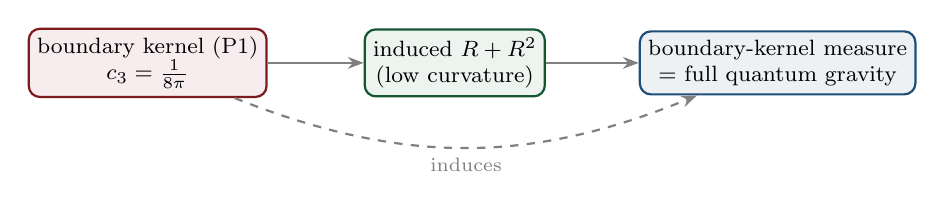
\begin{tikzpicture}[font=\footnotesize,
  b/.style={rectangle,rounded corners,draw,thick,align=center,inner sep=3pt,minimum height=8mm},
  ar/.style={-{Stealth[length=2mm]},thick,gray}]
  \node[b,draw=tfred!80!black,fill=tfred!8] (p1) at (0,0) {boundary kernel (P1)\\$\cthree=\tfrac1{8\pi}$};
  \node[b,draw=tfgreen!70!black,fill=tfgreen!8] (r2) at (3.9,0) {induced $R+R^2$\\(low curvature)};
  \node[b,draw=tfblue,fill=tfblue!8] (os) at (8.0,0) {boundary-kernel measure\\$=$ full quantum gravity};
  \draw[ar] (p1)--(r2); \draw[ar] (r2)--(os);
  \draw[ar,dashed] (p1) to[bend right=22] node[below,font=\scriptsize]{induces} (os);
\end{tikzpicture}
\end{center}

\begin{keybox}[Honest status of quantum gravity --- physical sector closed, ambient gap-decoupled \tF/\tA]
``Full quantum gravity beyond the $R^2$ sector'' is, in TFPT, \emph{not} a separate graviton-quantisation
programme: it is the well-definedness of the \emph{boundary-kernel path-integral measure} extended to the
dynamical metric beyond the FRW/minisuperspace reduction. Two results sharpen its status.
\textbf{(i) Heat-kernel grounded (G2).} The spectral action $\operatorname{Tr}f(D/\Lambda)$ gives, via the
standard Seeley--DeWitt coefficients for the Dirac operator ($a_2\!\sim\!-R/3$, $a_4|_{R^2}\!\sim\!R^2/72$),
Einstein--Hilbert $+$ $R^2$ \emph{structurally} --- the $R+R^2$ form is not postulated; the scalaron ratio
$M^2/\Mpl^2=6(4\pi)^2/f_0$ with the TFPT closure $\cthree^7$ fixing the cutoff moment $f_0$.
\textbf{(ii) Gap-decoupled (G5).} The metric coupling is gap-dominated,
$2\|V_{\mathrm{metric}}\|=0.785<\Delta=6\log\tfrac32=2.433$, so the admissible sector keeps a strictly
positive effective gap $\Delta_{\mathrm{eff}}=1.648>0$ under the stated RP and metric-coupling assumptions.
A positive gap protects the admissible IR sector from the un-built ambient, so under those assumptions the
admissible-sector measure is closed. \textbf{What remains \tA:} the ambient metric measure --- the
projective limit (G6) --- is the $G_{\mathrm{metric}}$ research gate; we do \emph{not} claim it is
physically irrelevant (that would itself be a physical interpretation), only that it is decoupled from the
admissible IR sector under the stated assumptions. \veri{v36\_spectral\_action\_g2.py}
\end{keybox}

% =====================================================================
\section*{Summary}
% =====================================================================
\addcontentsline{toc}{section}{Summary}
\begin{center}\small
\renewcommand{\arraystretch}{1.25}
\begin{tabularx}{\linewidth}{@{}p{2.9cm}cY@{}}
\toprule
\textbf{Item} & \textbf{Status} & \textbf{Honest handle / what is missing} \\
\midrule
$\eta_B$ & \tP & downstream readout $=6.1{\times}10^{-10}$ from closed $\Omega_b h^2$; leptogenesis is an interface (Boltzmann) \\
$m_p/m_e$ & \tA & cross-sector (QCD scale / closed $m_e$); scheme-level, not a compiler power \\
Koide $Q$ & \tP & computed $Q=0.664$, $0.33\%$ from $2/3$; near, not exact --- not tuned \\
dark matter & \tP/\tA & determinant-line axion candidate fixed, $\theta_i=170^\circ$ closed; relic scale $f_a,m_a$ open \\
quantum gravity & \tF/\tA & $R+R^2$ heat-kernel grounded (G2); physical sector gap-decoupled; only ambient limit (G6) open \\
\bottomrule
\end{tabularx}
\end{center}
\markerkey

\noindent\textbf{Net (honest).} Two of the five have a genuine quantitative handle that already lands on
the data ($\eta_B=6.1\times10^{-10}$ via the closed $\Omega_b$; the axion DM candidate with a closed
misalignment angle). One is a computed \emph{near}-miss reported without tuning (Koide $0.664$ vs $2/3$).
One is structural-only and left open ($m_p/m_e$ as a cross-sector ratio); quantum gravity has been
sharpened --- its $R+R^2$ form is now heat-kernel grounded (G2) and its physical sector is gap-decoupled
(G5), leaving only the ambient projective limit (G6) as a mathematical-completeness item. None has been
forced onto the compiler ladder --- which is exactly the right call: the strong results stay strong
precisely because the weak ones are not oversold.

% =====================================================================
\section*{Appendix: computational verification}
\addcontentsline{toc}{section}{Appendix: computational verification}
% =====================================================================
These are the \emph{frontier} items: most carry \tA\ (open) or \tP\ (conditional) and are therefore
\emph{not} part of the pass/fail suite. The one quantitative handle that is reproduced is
$\Omega_b{=}(1{-}\tfrac1{4\pi})\phiz$ (whence the $\eta_B$ order) in
\texttt{verification/v7\_gravity\_cosmo.py}. The $R+R^2$ structure and the gap-decoupling of the physical
QG sector \emph{are} machine-checked (\texttt{v28\_gravity\_fR.py}, \texttt{v36\_spectral\_action\_g2.py});
only the proton/electron ratio and the ambient projective limit (G6) are left open by design --- no script
``proves'' those, consistent with their \tA\ marking. The compiler/SM
identities they build on are checked by the suite in \texttt{verification/} (run
\texttt{python verification/run\_all.py}; see \texttt{verification/README.md}).

\end{document}
